\section{Moduł gracza}

Biblioteka stanowi zbiór funkcji wspomagających komunikację z grą oraz tworzenie tabel i wykresów. Funkcje te działają zarówno w środowisku Matlab jak i Octave.

\paragraph{SendData} \hspace{0pt} \\
Wysłanie danych na serwer.

\begin{lstlisting}[style=Matlab-editor]
txt = SendData(IPAddressSend,portSend,data,name, args)
\end{lstlisting}

Opis:
\begin{itemize}
\item  IPAddressSend -- adres ip serwera,
\item  portSend -- port serwera,
\item  data -- data packet sent to the server,
\item  name  -- określa sposób interpretowania danych,
\item  args  -- argumenty związane z informacjami sterującymi.
\end{itemize}

Zwraca odpowiedź serwera w formacie XML.

\paragraph{NumberToName} \hspace{0pt} \\
Zastępuje liczby reprezentującą typy pól ich nazwami.
\begin{lstlisting}[style=Matlab-editor]
result = NumberToName(array, names)
\end{lstlisting}

Opis:
\begin{itemize}
\item  array -- tabela zawierająca informacje o mapie,
\item  names -- nazwy pól mapy.
\end{itemize}

Zwraca tabelę zawierającą informacje o mapie.

\paragraph{ChangeBeginEnd} \hspace{0pt} \\
Oznaczanie początków i końców ścieżek.
\begin{lstlisting}[style=Matlab-editor]
result = ChangeBeginEnd(array)
\end{lstlisting}

Opis:
\begin{itemize}
\item  array -- tabela zawierająca informacje o mapie.
\end{itemize}

Zwraca tabelę zawierającą informacje o mapie.

\paragraph{TilemapToXML} \hspace{0pt} \\
Konwersja mapy z tablicy do formatu XML.
\begin{lstlisting}[style=Matlab-editor]
txt = TilemapToXML(tilemap)
\end{lstlisting}

Opis:
\begin{itemize}
\item  tilemap -- mapa w postaci tablicy.
\end{itemize}

Zwraca mapę zapisaną w formacie xml.

Przykład przesłania do gry polecenia utworzenia planszy:
\begin{lstlisting}[style=Matlab-editor]
%Adres serwera
IPAddressSend = '127.0.0.1';
%Port na ktorym nasluchuje serwer
portSend = 55001;
%Tablica reprezentujaca plansze gry w ktorej liczby reprezentuja typy kafelkow (1 - ziemia, 2 - woda bedaca elementem sciezki ruchu przeciwnikow, 3 - poczatek sciezki, 4 - koniec sciezki) 
tilemap = [1	3	1	3	1	1	1	1	1	1	1	3	1	1	1 1;
           	1	2	1	2	1	1	1	1	1	1	1	2	1	1	1 1;
           	1	2	1	2	1	1	1	1	3	1	2	2	1	1	1 1;
           	1	2	1	2	1	1	1	1	2	1	2	1	1	1	1 1;
           	1	2	1	2	1	1	1	1	2	1	2	1	1	1	1 1;
           	1	2	1	2	2	1	1	1	2	1	2	2	1	1	1 1;
           	1	2	1	1	2	1	1	2	2	1	1	2	1	1	1 1;
           	1	2	1	2	2	1	1	2	1	1	2	2	1	1	1 1;
           	1	2	1	2	1	1	1	2	1	1	2	1	1	1	1 1;
           	1	2	1	2	1	1	1	2	2	1	2	2	2	2	1 1;
           	1	2	1	2	1	1	1	1	2	1	1	1	1	2	2 1;
           	1	2	1	2	2	1	1	1	2	2	4	1	1	1	2 1;
           	1	4	1	1	4	1	1	1	1	1	1	1	1	1	4 1];
%Nazwy typow kafelkow. Pozycja w tablicy odpowiada numerowi z tablicy tilemap
names{1} = 'Ground';
names{2} = 'Water';
names{3} = 'Begin';
names{4} = 'End';
%Obrot tablicy tak aby orientacja tablicy odpowiadala orientacji planszy w grze
tilemap = rot90(rot90(rot90(tilemap)));
% Zamiana tablicy na tablice struktur z nazwami kafekow zamiast numerow
tilemapNames = NumberToName(tilemap,names);
%Zamiana nazw kafelkow Begin i End na Water. Przypisanie tym kafelkom oznaczenia poczatku lub konca sciezki.
tilemapNames = ChangeBeginEnd(tilemapNames);
%Zamiana tablicy sturktur na tekst w formacie xml.
txt = TilemapToXML(tilemapNames);
%Wyslanie polecenia utworzenia nowej planszy (Tilemap) oraz danych w formacie xml do gry.
SendData(IPAddressSend,portSend,txt,'Tilemap',[]);
\end{lstlisting}

\paragraph{Char2Code} \hspace{0pt} \\
Zastępowanie kodów znaków kodami używanymi przez maszynę.
\begin{lstlisting}[style=Matlab-editor]
machineCode = Char2Code(code)
\end{lstlisting}

Opis:
\begin{itemize}
\item code -- kod znaku.
\end{itemize}

Zwraca kody automatu.

Przykład odczytu i dekodowania pliku xml:
\begin{lstlisting}[style=Matlab-editor]
%Konwersja znaku
code = Char2Code('a');
\end{lstlisting}

\paragraph{Machine} \hspace{0pt} \\
Automat dzielący tekst na elementy i przypisujący im kody końcowych stanów maszyny.
\begin{lstlisting}[style=Matlab-editor]
result = Machine(data,t)
\end{lstlisting}

Opis:
\begin{itemize}
\item data -- tekst,
\item t -- tabela przejść pomiędzy stanami automatu.
\end{itemize}

Zwraca tablicę struktur zawierającą fragment tekstu (pole txt) i przypisany do niego stan (pole stanu).

Przykład odczytu i dekodowania pliku xml:
\begin{lstlisting}[style=Matlab-editor]
%Odczyt pliku xml
dataTower = fileread('towers.xml');
%Definicja tablicy stanow
t = zeros(11,24);
t(1,1) = 1;t(2,1) = 17;t(3,1) = 2;t(4,1) = 8;t(5,1) = 12;t(6,1) = 4;t(8,1) = 6;t(9,1) = 15;t(10,1) = 22;
t(:,2) = 3;t(5,2) = 10;t(10,2) = 20;
t(1,4) = 5;t(2,4) = 5;t(4,4) = 5;t(5,4) = 5;t(6,4) = 4;t(7,4) = 4;t(9,4) = 5;
t(:,6) = 6;t(8,6) = 7;
t(:,7) = 19;
t(:,8) = 9;
t(:,10) = 11;
t(4,12) = 13;
t(:,13) = 14;
t(:,15) = 16;
t(:,17) = 18;
t(:,20) = 21;
t(4,22) = 23;
t(:,23) = 24;
%Analiza pliku
result = Machine(dataTower,t);
\end{lstlisting}

W zmiennej result znajduje się tablica struktur zawierajęca tekst i numer stanu mu przypisany. 

\paragraph{ParseXML} \hspace{0pt} \\
Analizuje tekst zawierający plik XML.
\begin{lstlisting}[style=Matlab-editor]
result = ParseXML(data)
\end{lstlisting}

Opis:
\begin{itemize}
\item data -- tablica tekstowa zawierająca dane w formacie XML.
\end{itemize}

Zwraca tablicę struktur, których struktura odzwierciedla strukturę danych XML, nazwami pól są nazwy elementów XML.

Przykład odczytania i zdekodowania pliku xml:
\begin{lstlisting}[style=Matlab-editor]
%Odczytanie pliku xml
dataTower = fileread('towers.xml');
%Konwersja pliku xml
dataTower = ParseXML(dataTower);
\end{lstlisting}

Zawartość pliku towers.xml:
\lstinputlisting[language=XML]{xml/towersBib.xml}

Plik towers.xml zawiera współrzędne wież i ich numery porządkowe. Przykład dostępu do tych danych:
\begin{lstlisting}[style=Matlab-editor]
x=dataTower.Answer.TowerCoordinates{1}.Element{i}.x;
y=dataTower.Answer.TowerCoordinates{1}.Element{i}.y;
no=dataTower.Answer.TowerCoordinates{1}.Element{i}.no;
\end{lstlisting}

\paragraph{GetVectorFromCell} \hspace{0pt} \\
Odczyt wektora danych z wybranego pola tablicy struktury.
\begin{lstlisting}[style=Matlab-editor]
res = GetVectorFromCell(data, field)
\end{lstlisting}

Opis:
\begin{itemize}
\item data -- tablica struktur,
\item field -- odczytywane pola struktury.
\end{itemize}

Zwraca wektor danych.

Przykład odczytania współrzędnych x wież jako tablicy:
\begin{lstlisting}[style=Matlab-editor]
%Odczytanie pliku xml
dataTower = fileread('towers.xml');
%Konwersja pliku xml
dataTower = ParseXML(dataTower);
%Odczytanie wspolrzednych x wiez jako tablicy
x = GetVectorFromCell(dataTower.Answer.TowerCoordinates{1}.Element,'x');
\end{lstlisting}

Zawartość pliku towers.xml:
\lstinputlisting[language=XML]{xml/towersBib.xml}

\paragraph{SetEnemies} \hspace{0pt} \\
Tworzenie informacji w formie XML o konkretnym typie przeciwnika.
\begin{lstlisting}[style=Matlab-editor]
txt = SetEnemies(count,speed,startHealth,armour,cost,destroyCoins,coinsToEnd,type,tag)
\end{lstlisting}

Opis:
\begin{itemize}
\item count -- maksymalna liczba przeciwników,
\item speed -- prędkość przeciwnika,
\item startHealth -- początkowa wartość życia przeciwnika,
\item armour -- zbroja wroga (odporność na kule),
\item cost -- koszt stworzenia i wysłania wroga,
\item destroyCoins -- zysk dla zarządcy wież za zestrzelenie wroga,
\item coinsToEnd -- zysk dla menadżera przeciwników, jeśli dotrze on do końca ścieżki,
\item type -- typ przeciwnika,
\item tag -- nazwa typu obiektu.
\end{itemize}

Zwraca informacje zapisane w formacie xml.

Przykład przesłania do gry polecenia utworzenia nowego typu przeciwnika:
\begin{lstlisting}[style=Matlab-editor]
%Adres serwera
IPAddressSend = '127.0.0.1';
%Port na ktorym nasluchuje serwer
portSend = 55001;
%Utworzenie danych w formacie xml dotyczacych nowego typu przeciwnika
txt = SetEnemies(-1,2,20,2,30,30,40,'Paper','Enemy');
%Wyslanie polecenia (Command) utworzenia nowego typu przeciwnika (SetEnemies)
SendData(IPAddressSend,portSend,txt,'Command','name="SetEnemies"');
\end{lstlisting}

\paragraph{SetTowers} \hspace{0pt} \\
Tworzenie informacji w formie XML o konkretnym typie wieży
\begin{lstlisting}[style=Matlab-editor]
txt = SetTowers(count,speed,rateOfFire,force,bulletStrength,cost,type,tag)
\end{lstlisting}

Opis:
\begin{itemize}
\item count -- maksymalna liczba wież,
\item speed -- prędkość obrotu wież,
\item rateOfFire -- szybkostrzelność wież,
\item force -- siła ognia wieży (określa zasięg),
\item bulletStrength -- siła pocisku wieży (wpływa na liczbę ran zadanych wrogowi),
\item cost -- koszt stworzenia wieży,
\item type -- typ wieży,
\item tag -- typ obiektu, który zaatakuje wieża.
\end{itemize}

Zwraca informacje zapisane w formacie xml.

Przykład przesłania do gry polecenia utworzenia nowego typu wieży:
\begin{lstlisting}[style=Matlab-editor]
%Adres serwera
IPAddressSend = '127.0.0.1';
%Port na ktorym nasluchuje serwer
portSend = 55001;
%Utworzenie danych w formacie xml dotyczacych nowego typu wiezy
txt = SetTowers(-10,1000,1,1000,5,10,'Tower','Enemy');
%Wyslanie polecenia (Command) utworzenia nowego typu wiezy (SetTowers)
SendData(IPAddressSend,portSend,txt,'Command','name="SetTowers"');
\end{lstlisting}

\paragraph{StartEnemy} \hspace{0pt} \\

Tworzenie przeciwnika i wysyłanie go wybraną ścieżką.
\begin{lstlisting}[style=Matlab-editor]
txt = StartEnemy(beginNo,endNo)
\end{lstlisting}

Description:
\begin{itemize}
\item beginNo -- numer punktu początkowego,
\item endNo -- numer punktu końcowego.
\end{itemize}

Zwraca informacje zapisane w formacie xml.

Przykład utworzenia przeciwnika i wysłania go z punktu startowego 1 do punktu końcowego 3: 
\begin{lstlisting}[style=Matlab-editor]
%Adres serwera
IPAddressSend = '127.0.0.1';
%Port na ktorym nasluchuje serwer
portSend = 55001;
%Utworzenie danych w formacie xml zawierajacych informacje o punkcie startowym i koncowym
txt = StartEnemy(1,3);
%Wyslanie polecenia (Command) utworzenia przeciwnika i wyslania go od wskazanego punktu startowego do wskazanego punktu koncowego (StartEnemy)
errorStartEnemy = SendData(IPAddressSend,portSend,txt,'Command','name="StartEnemy"');
\end{lstlisting}

\paragraph{AddTower} \hspace{0pt} \\

Dodanie wieży.
\begin{lstlisting}[style=Matlab-editor]
txt = AddTower(noTower,x,y)
\end{lstlisting}

Opis:
\begin{itemize}
\item noTower -- numer wieży,
\item x -- współrzędna x wieży,
\item y -- współrzędna y wieży.
\end{itemize}

Zwraca informacje zapisane w formacie xml.

Przykład dodania wieży o numerze 3 w miejsce o współrzędnych $x=1$, $y = 4$: 
\begin{lstlisting}[style=Matlab-editor]
%Adres serwera
IPAddressSend = '127.0.0.1';
%Port na ktorym nasluchuje serwer
portSend = 55001;
%Utworzenie danych w formacie xml zawierajacych informacje o numerze wiezy i jej wspolrzednych
txt = AddTower(3,1,4);
%Wyslanie polecenia (Command) utworzenia wiezy (AddTower)
errorAddTower = SendData(IPAddressSend,portSend,txt,'Command','name="AddTower"');
\end{lstlisting}

\paragraph{RemoveCriteria} \hspace{0pt} \\
Usunięcie kryteriów, których wartości dla wszystkich wariantów decyzyjnych nie różnią się od siebie.

\begin{lstlisting}[style=Matlab-editor]
[E,W,PrefDirection, ind] = RemoveCriteria(E,W,PrefDirection)
\end{lstlisting}

Opis:
\begin{itemize}
\item E -- tabela danych, kolumny są kryteriami, a wiersze alternatywami,
\item W -- wagi kryteriów,
\item PrefDirection -- kryteria Kierunek preferencji (1-max;2-min),
\item ind -- indeksy kryteriów, które nie zostały usunięte.
\end{itemize}

Zwraca tabelę danych, kolumny są kryteriami, a wiersze alternatywami.

Przykład usuwania kryteriów:
\begin{lstlisting}[style=Matlab-editor]
%Tablica danych
E =[12    3    1   13    1    1;
       15    0    0   13    1    1;
       13    0    0   13    1    1;
       19    0    0   13    1    1];
%Wektor wag kryteriow
W=[2 10 8 1 20 10];
%Wektor kierunkow preferencji kryteriow: 1-max, 2-min
PrefDirection=[2 2 2 2 1 1];
%Usuniecie kryteriow, aktualizowana jest tablica danych oraz wektory wag i kierunkow preferencji
[E,W,PrefDirection, ind] = RemoveCriteria(E,W,PrefDirection)
\end{lstlisting}

\paragraph{TOPSIS} \hspace{0pt} \\
Funkcja TOPIS. Oblicza wartości miary alternatyw metodą TOPSIS.

\begin{lstlisting}[style=Matlab-editor]
S=TOPSIS(E,W,PrefDirection,p)
\end{lstlisting}

Opis:
\begin{itemize}
\item E -- tabela danych, kolumny są kryteriami, a wiersze alternatywami,
\item W -- wagi kryteriów,
\item PrefDirection -- kierunek preferencji kryteriów (1-max;2-min),
\item p -- współczynnik.
\end{itemize}

Zwraca tablicę wartości miar dla wariantów decyzji.

Przykład obliczania wartości miary:
\begin{lstlisting}[style=Matlab-editor]
%Tablica danych
E = [12    3    1;
       15    0    0;
       13    0    0;
       19    0    0];
%Wektor wag kryteriow
W=[2 10 8];
%Wektor kierunkow preferencji kryteriow: 1-max, 2-min
PrefDirection=[2 2 2];
%Obliczanie wartosci miary
score=TOPSIS(E,W,PrefDirection,p);
\end{lstlisting}

\paragraph{VIKOR} \hspace{0pt} \\
Funkcja VIKOR. Oblicza wartości miary alternatyw metodą VIKOR.

\begin{lstlisting}[style=Matlab-editor]
[Q,S,R]=VIKOR(E,W,PrefDirection,q)
\end{lstlisting}

Opis:
\begin{itemize}
\item E -- tabela danych, kolumny są kryteriami, a wiersze alternatywami,
\item W -- wagi kryteriów,
\item PrefDirection -- kierunek preferencji kryteriów (1-max;2-min),
\item p -- współczynnik.
\end{itemize}

Returns an array of measure values for decision variants.

Przykład obliczenia wartości miary:
\begin{lstlisting}[style=Matlab-editor]
%Tablica danych
E = [12    3    1;
       15    0    0;
       13    0    0;
       19    0    0];
%Wektor wag kryteriow
W=[2 10 8];
%Wektor kierunkow preferencji kryteriow: 1-max, 2-min
PrefDirection=[2 2 2];
%Obliczenie trzech typow wartosci miary
[Q,S,R]=VIKOR(E,W,PrefDirection,p);
\end{lstlisting}


\paragraph{GenerateRanking} \hspace{0pt} \\
Tworzy ranking alternatyw.

\begin{lstlisting}[style=Matlab-editor]
ranking = GenerateRanking(v)
\end{lstlisting}

Opis:
\begin{itemize}
\item  v -- Wektor ocen alternatyw.
\end{itemize}

Returns ranking positions.

Example of creating a ranking:
\begin{lstlisting}[style=Matlab-editor]
%Przykladowy wektor
exampleVector = [1.25 2.23 1.25 0.3 1.5 4.5];
%Utworzenie rankingu
ranking = GenerateRanking(exampleVector);
\end{lstlisting}

\paragraph{GenerateReport} \hspace{0pt} \\
Generowanie raportu z wynikami testowanej metody MCDA.

\begin{lstlisting}[style=Matlab-editor]
ranking = GenerateReport(fileNamePlot,fileNameTab,scoreArray,funName,EnemiesToEnd,EnemiesMeanHealthRatio,TracksCost);
\end{lstlisting}

Description:
\begin{itemize}
\item fileNamePlot -- nazwa pliku, do którego zostanie zapisany wykres,
\item fileNameTab -- nazwa pliku, do którego zostanie zapisana tabela,
\item scoreArray -- ocenia (oceny) ścieżki,
\item funName -- nazwa testowanej metody MCDA,
\item EnemiesToEnd -- liczba wrogów, którzy dotarli do końca wszystkich ścieżek (główny wynik metody MCDA),
\item EnemiesMeanHealthRatio -- średni poziom zdrowia wrogów, którzy dotarli do końca ścieżek (dodatkowy wynik metody MCDA),
\item TracksCost -- całkowita długość ścieżek wybranych metodą MCDA (drugi dodatkowy wynik metody MCDA).
\end{itemize}

Przykład generowania raportu:
\begin{lstlisting}[style=Matlab-editor]
%Tablica zawierajaca przykladowe (hipotetyczne) wyniki wyboru sciezki metoda MCDA w grze skladajacej sie z czterech rund z dwiema sciezkami do wyboru
exampleArray = [0.5 0.4;
  0.3 0.4;
  0.7 0.3;
  0.6 0.8];
%Zmienne zawierajace przykladowe (hipotetyczne) wyniki metody MCDA
exampleEnemiesToEnd = 3;
exampleEnemiesMeanHealthRatio = 0.65;
exampleTracksCost = 56;
%Tworzenie raportu z gry z wynikami metody MCDA
GenerateReport('scoreRounds.png','scoreRound.html',exampleArray,'TOPSIS',exampleEnemiesToEnd,exampleEnemiesMeanHealthRatio,exampleTracksCost);
\end{lstlisting}

Zawartość pliku 'scoreRounds.html':
\lstinputlisting[language=HTML5]{html/scoreRound.html}

Rysunek~\ref{Fig:scoreRoundshtml} przedstawia zrzut ekranu przedstawiający wygląd wygenerowanej strony.

\begin{figure}
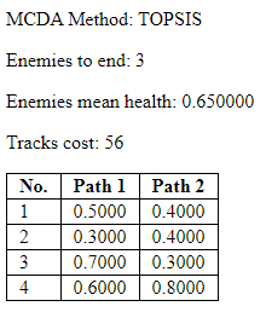
\includegraphics[width=4cm]{images/scoreRoundshtml.png}
\caption{Wizualizacja wygenerowanej strony html}
\label{Fig:scoreRoundshtml}
\end{figure} 

Rysunek~\ref{Fig:scoreRounds} przedstawia zawartość pliku 'scoreRounds.png'.

\begin{figure}
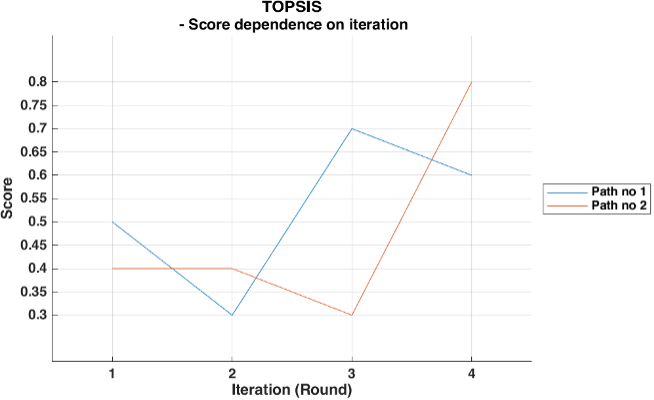
\includegraphics[width=10cm]{images/scoreRounds.png}
\caption{Zawartość pliku 'scoreRounds.png'}
\label{Fig:scoreRounds}
\end{figure} 

\paragraph{GenerateTabular} \hspace{0pt} \\
Generowanie tabeli typu tabular.
\begin{lstlisting}[style=Matlab-editor]
GenerateTabular(fileName,data,columnDescriptions,rowDescriptions,rowsBold,decimalPlaces)
\end{lstlisting}

Opis:
\begin{itemize}
\item fileName -- nazwa pliku, do którego zostanie zapisana tablica,
\item data -- zapisana tablica,
\item columnDescriptions -- opisy kolumn,
\item rowDescriptions -- opisy wierszy, pusta tablica([]) oznacza brak opisów,
\item rowsBold -- 0 oznacza, że opisy wierszy tabeli nie są pogrubione, a 1 oznacza że są pogrubione,
\item decimalPlaces -- liczba miejsc po przecinku.
\end{itemize}

Przykład generowania tablicy: 
\begin{lstlisting}[style=Matlab-editor]
%Tablica
exampleArray = [1 2;
                  3 1;
                  5 2;
                  2 4];
%Opisy kolumn
columnDescriptions={'No','Data 1','Data 2'};
%Opisy wierszy
rowDescriptions={'1','2','3','4'};
%Utworzenie pliku zawierajacego srodowisko tablular
GenerateTabular('array.tex',exampleArray,columnDescriptions,rowDescriptions,0,0);
\end{lstlisting}

Zawartość pliku array.tex:
\lstinputlisting[style=lstStyleLaTeX]{table/array.tex}

Tablicę można dołączyć do pliku Latex-a: 
\begin{lstlisting}[style=lstStyleLaTeX]
\begin{table}
\begin{tikzpicture}
\begin{axis}[
    title={Example},
    xlabel={No},
    ylabel={Data},
    legend pos=outer north east,
    ymajorgrids=true,
    grid style=dashed,
]

\addplot[
    color=blue,
    mark=square
    ]
    table[x=No,y=D1]
    {fig/array.dat};
\addplot[
    color=red,
    mark=square
    ]
    table[x=No,y=D2]
    {fig/array.dat};

    \legend{Data 1, Data 2}

\end{axis}
\end{tikzpicture}

\caption{Wygenerowana tablica}
\end{table}
\end{lstlisting}

Uzyskany efekt przedstawia tablica~\ref{array}.

\begin{table}
\begin{tikzpicture}
\begin{axis}[
    title={Example},
    xlabel={No},
    ylabel={Data},
    legend pos=outer north east,
    ymajorgrids=true,
    grid style=dashed,
]

\addplot[
    color=blue,
    mark=square
    ]
    table[x=No,y=D1]
    {fig/array.dat};
\addplot[
    color=red,
    mark=square
    ]
    table[x=No,y=D2]
    {fig/array.dat};

    \legend{Data 1, Data 2}

\end{axis}
\end{tikzpicture}

\caption{Wygenerowana tablica}
\label{array}
\end{table}

\paragraph{GenerateTikzData} \hspace{0pt} \\
Generowanie plików danych dla wykresów Tikz.
\begin{lstlisting}[style=Matlab-editor]
GenerateTikzData(fileName,data,columnDescriptions)
\end{lstlisting}

Opis:
\begin{itemize}
\item fileName -- nazwa pliku, do którego zostanie zapisana tablica,
\item data -- zapisywana tablica,
\item columnDescriptions -- opisy kolumn.
\end{itemize}

Przykład generowania danych: 
\begin{lstlisting}[style=Matlab-editor]
%Tablica
exampleArray = [1 2;
                  3 1;
                  5 2;
                  2 4];
%Opisy kolumn
columnDescriptions={'No','D1','D2'};
%Utworzenie pliku zawierajacego dane dla wykresow tikz
GenerateTikzData('array.dat',[[1:size(exampleArray,1)]' exampleArray],columnDescriptions);
\end{lstlisting}

Zawartość pliku array.dat:
\lstinputlisting{fig/array.dat}

Plik array.dat można dołączyć do wykresu tikz-a: 
\lstinputlisting[style=lstStyleLaTeX]{fig/array.tikz}

Uzyskany efekt przedstawia rysunek~\ref{Fig:array}.

\begin{figure}
\begin{tikzpicture}
\begin{axis}[
    title={Example},
    xlabel={No},
    ylabel={Data},
    legend pos=outer north east,
    ymajorgrids=true,
    grid style=dashed,
]

\addplot[
    color=blue,
    mark=square
    ]
    table[x=No,y=D1]
    {fig/array.dat};
\addplot[
    color=red,
    mark=square
    ]
    table[x=No,y=D2]
    {fig/array.dat};

    \legend{Data 1, Data 2}

\end{axis}
\end{tikzpicture}

\caption{Wykres na podstawie danych wygenerowanych przez funkcję GenerateTikzData}
\label{Fig:array}
\end{figure}


